\chapter{Oscillatore armonico smorzato}
% (richiede: \usepackage{tikz} \usetikzlibrary{arrows.meta,decorations.pathmorphing})


\textbf{Punto materiale su molla con attrito viscoso}

Consideriamo un punto materiale di massa \(m\) vincolato a muoversi su una retta, collegato a una molla (costante elastica \(k\)) e soggetto ad attrito viscoso (coefficiente \(\tilde{\gamma}\)). Indichiamo con \(x(t)\) lo spostamento dalla posizione di equilibrio, con \(v(t)=\dot x(t)\) la velocità.

\begin{figure}
\centering
\begin{tikzpicture}[>=Latex,scale=1.0]
  % asse
  \draw[->] (-0.3,0) -- (7.0,0);

  % parete
  \draw[thick] (0, -0.7) -- (0, 0.7);
  \draw[thick] (-0.25, -0.7) -- (-0.25, 0.7);
  \foreach \y in {-0.65,-0.45,...,0.65} {
    \draw[thick] (-0.25,\y) -- (0,\y+0.2);
  }

  % punto di equilibrio
  \fill (0.1,0) circle (1.2pt);
  \node[below] at (0.15,0) {$0$};

  % massa
  \draw[thick] (5.2,-0.35) rectangle (6.0,0.35);
  \node at (5.6,0) {$m$};

  % molla
  \draw[thick,decorate,decoration={coil,aspect=0.7,segment length=6pt,amplitude=4pt}]
    (0,0) -- (5.2,0);

  % frecce forze
  \draw[->,thick,green!60!black] (5.6,0.55) -- (4.7,0.55);
  \node[green!60!black,above] at (5.15,0.55) {$F_{\mathrm{el}}$};

  \draw[->,thick,red!70!black] (5.6,-0.55) -- (4.7,-0.55);
  \node[red!70!black,below] at (5.15,-0.55) {$F_{\mathrm{av}}$};

  % velocità e spostamento
  \draw[->,thick,orange!80!black] (6.05,0.0) -- (6.75,0.0);
  \node[orange!80!black,right] at (6.75,0.0) {$v$};

  \draw[|-|] (0,-1.1) -- (5.6,-1.1);
  \node[below] at (2.8,-1.1) {$x(t)$};
\end{tikzpicture}
\caption{Massa \(m\) collegata a molla e attrito viscoso.}
\end{figure}

\medskip
\textbf{Forze in gioco.}
\begin{itemize}
  \item Forza elastica (legge di Hooke):
  \[
  F_{\mathrm{el}}=-k\,x(t).
  \]
  \item Forza di attrito viscoso:
  \[
  F_{\mathrm{av}}=-\tilde{\gamma}\,v(t)=-\tilde{\gamma}\,\dot x(t).
  \]
\end{itemize}

\textbf{Equazione di Newton.}
Lungo la direzione del moto vale
\[
\sum F = m a \qquad \Longrightarrow \qquad m\,\ddot x(t)=F_{\mathrm{el}}+F_{\mathrm{av}}.
\]
Sostituendo le espressioni delle forze:
\[
m\,\ddot x(t)=-k\,x(t)-\tilde{\gamma}\,\dot x(t).
\]
Dividendo per \(m\):
\[
\ddot x(t)+\frac{\tilde{\gamma}}{m}\,\dot x(t)+\frac{k}{m}\,x(t)=0.
\]

\textbf{Notazioni standard.}
Definiamo
\[
\omega^2=\frac{k}{m},
\qquad
2\gamma=\frac{\tilde{\gamma}}{m}.
\]
Otteniamo infine l’equazione dell’oscillatore armonico smorzato:
\[
\ddot x(t)+2\gamma\,\dot x(t)+\omega^2 x(t)=0.
\]


Nel \textbf{caso (i)} assumiamo
\[
\gamma^2>\omega^2,
\]
quindi le radici dell'equazione caratteristica saranno \emph{reali e distinte}.
\medskip

\inizioapprof

\textbf{Spazio delle soluzioni (campo scalare).}

L'operatore differenziale
\[
L[x]=\ddot x+2\gamma \dot x+\omega^2 x
\]
è lineare. Di conseguenza, l'insieme delle soluzioni reali
\[
\mathcal S_{\mathbb R}
=
\{x:I\to\mathbb R \mid x\in C^2,\ L[x]=0\}
\]
è uno spazio vettoriale su \(\mathbb R\). Inoltre, per teoria standard delle ODE,
\[
\dim_{\mathbb R}(\mathcal S_{\mathbb R})=2:
\]
basta trovare due soluzioni reali linearmente indipendenti per descrivere tutte le soluzioni.

\fineapprof

\medskip

Poiché l'equazione è lineare omogenea a coefficienti costanti, proviamo una soluzione del tipo
\[
x(t)=e^{\lambda t},
\]
con \(\lambda\in\mathbb{C}\). Sostituendo:
\[
\dot x(t)=\lambda e^{\lambda t},
\qquad
\ddot x(t)=\lambda^2 e^{\lambda t}.
\]
Allora
\[
\lambda^2 e^{\lambda t}+2\gamma \lambda e^{\lambda t}+\omega^2 e^{\lambda t}=0.
\]
Poiché \(e^{\lambda t}\neq 0\) per ogni \(t\), otteniamo l'equazione caratteristica
\[
\lambda^2+2\gamma\lambda+\omega^2=0.
\]
Le radici sono
\[
\lambda_{\pm}=-\gamma\pm\sqrt{\gamma^2-\omega^2}.
\]
Nel caso (a) \(\gamma^2-\omega^2>0\), quindi \(\lambda_+\neq \lambda_-\) e \(\lambda_\pm\in\mathbb{R}\).

\medskip
\textbf{Soluzioni fondamentali e combinazione lineare.}
Le funzioni
\[
x_+(t)=e^{\lambda_+ t},
\qquad
x_-(t)=e^{\lambda_- t}
\]
sono due soluzioni reali dell'equazione. Essendo \(\lambda_+\neq\lambda_-\), esse sono linearmente indipendenti su \(\mathbb{R}\).
Per linearità, ogni combinazione lineare reale è ancora soluzione; dunque la soluzione reale generale è
\[
x(t)=A e^{\lambda_+ t}+B e^{\lambda_- t},
\qquad A,B\in\mathbb{R}.
\]

\medskip
\textbf{Nota su esistenza e unicità (dati iniziali reali).}
Assegnati \(x(0)=x_0\in\mathbb{R}\) e \(\dot x(0)=v_0\in\mathbb{R}\), il teorema di Cauchy garantisce esistenza e unicità di una soluzione reale.
In questo caso, la scelta di \(A,B\in\mathbb{R}\) permette di soddisfare univocamente le condizioni iniziali.

\medskip
\textbf{Comportamento asintotico.}
Poiché
\[
\lambda_-=-\gamma-\sqrt{\gamma^2-\omega^2}<0,
\qquad
\lambda_+=-\gamma+\sqrt{\gamma^2-\omega^2}<0
\]
(essendo \(\sqrt{\gamma^2-\omega^2}<\gamma\)), entrambi i termini decadono esponenzialmente e quindi
\[
x(t)\to 0 \qquad \text{per } t\to+\infty.
\]
% Richiede: \usepackage{pgfplots} \pgfplotsset{compat=1.18}

\begin{center}
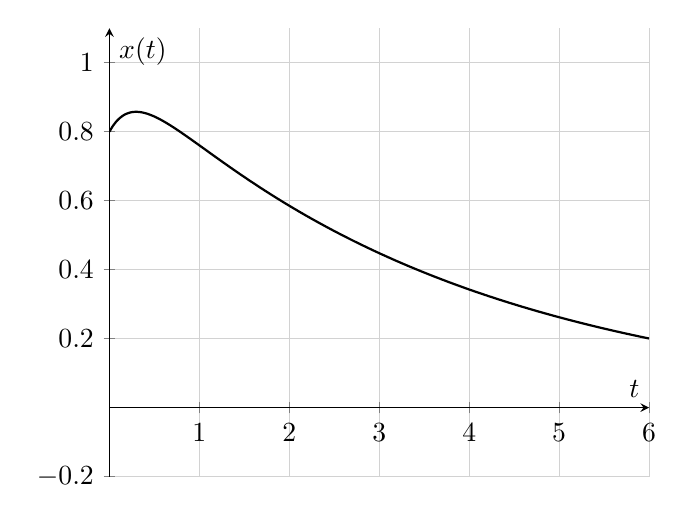
\begin{tikzpicture}
\begin{axis}[
  xlabel={$t$},
  ylabel={$x(t)$},
  axis lines=middle,
  xmin=0, xmax=6,
  ymin=-0.2, ymax=1.1,
  samples=300,
  domain=0:6,
  grid=both,
  grid style={line width=.1pt, draw=gray!25},
  major grid style={line width=.2pt, draw=gray!35},
]
% Caso (a) sovrasmorzato: gamma=2, omega=1 -> lambda_+=-2+sqrt(3), lambda_-=-2-sqrt(3)
% Esempio di soluzione: A=1, B=-0.2 (decadimento senza oscillazioni)
\addplot[thick] {1*exp((-2+sqrt(3))*x) - 0.2*exp((-2-sqrt(3))*x)};
\end{axis}
\end{tikzpicture}
\end{center}
% Richiede: \usepackage{tikz} \usepackage{pgfplots} \pgfplotsset{compat=1.18}


\textbf{Caso (ii): \(\gamma=0\) (oscillatore armonico non smorzato)}

Se \(\gamma=0\), l'equazione diventa
\[
\ddot x+\omega^2 x=0.
\]
Proviamo ancora \(x(t)=e^{\lambda t}\). Sostituendo:
\[
\lambda^2 e^{\lambda t}+\omega^2 e^{\lambda t}=0
\quad\Rightarrow\quad
\lambda^2+\omega^2=0
\quad\Rightarrow\quad
\lambda=\pm i\omega.
\]
Quindi due soluzioni (complesse) sono \(e^{i\omega t}\) ed \(e^{-i\omega t}\), e la soluzione generale (in \(\mathbb{C}\)) è
\[
x(t)=A e^{i\omega t}+B e^{-i\omega t}.
\]

Scriviamo \(A=A_r+iA_i\) e \(B=A_r-iA_i\) (così \(B=\overline{A}\) e \(x(t)\) risulta reale). Allora
\[
x(t)=(A_r+iA_i)e^{i\omega t}+(A_r-iA_i)e^{-i\omega t}.
\]
Usando la formula di Eulero
\[
e^{i\omega t}=\cos(\omega t)+i\sin(\omega t),
\qquad
e^{-i\omega t}=\cos(\omega t)-i\sin(\omega t),
\]
si ottiene
\[
x(t)=(A_r+iA_i)(\cos\omega t+i\sin\omega t)+(A_r-iA_i)(\cos\omega t-i\sin\omega t).
\]
Sviluppando e raccogliendo:
\[
x(t)=2A_r\cos(\omega t)-2A_i\sin(\omega t).
\]
Questa forma si può riscrivere come
\[
x(t)=C\cos(\omega t+\varphi),
\]
dove \(C\) è l'ampiezza e \(\varphi\) la fase (da determinare con le condizioni iniziali), mentre \(\omega\) è un parametro del sistema. Infatti possiamo scrivere
\[
x(t)=2A_r\cos(\omega t)-2A_i\sin(\omega t)
=\sqrt{4A_r^{\,2}+4A_i^{\,2}}
\left(
\frac{A_r}{\sqrt{A_r^{\,2}+A_i^{\,2}}}\cos(\omega t)
-\frac{A_i}{\sqrt{A_r^{\,2}+A_i^{\,2}}}\sin(\omega t)
\right)=
\]
\[
= C\cos(\omega t+\varphi)
\]

\[
\Rightarrow\
\cos\varphi=\frac{A_r}{\sqrt{A_r^{\,2}+A_i^{\,2}}},
\qquad
\sin\varphi=\frac{A_i}{\sqrt{A_r^{\,2}+A_i^{\,2}}},
\qquad
C=\sqrt{4A_r^{\,2}+4A_i^{\,2}}.
\]

\[
\sin\varphi,\ \cos\varphi,\ C\ \text{risultano ben definite perché}
\]

\[
Im\!\left(\frac{A_r}{\sqrt{A_r^{\,2}+A_i^{\,2}}}\right)=[-1,1],
\qquad
Im\!\left(\frac{A_i}{\sqrt{A_r^{\,2}+A_i^{\,2}}}\right)=[-1,1],
\]

\[
Im\!\left(\sqrt{4A_r^{\,2}+4A_i^{\,2}}\right)=[0,+\infty).
\]

Derivando:
\[
\dot x(t)=-C\omega \sin(\omega t+\varphi).
\]
In particolare, imponendo \(x(0)=x_0\) e \(\dot x(0)=v_0\),
\[
x_0=C\cos\varphi,
\qquad
v_0=-C\omega\sin\varphi.
\]
Quindi
\[
\frac{v_0}{x_0}=-\omega\tan\varphi
\quad\Rightarrow\quad
\varphi=\arctan\!\left(-\frac{v_0}{\omega x_0}\right),
\qquad
C=\frac{x_0}{\cos\varphi}.
\]

\begin{center}
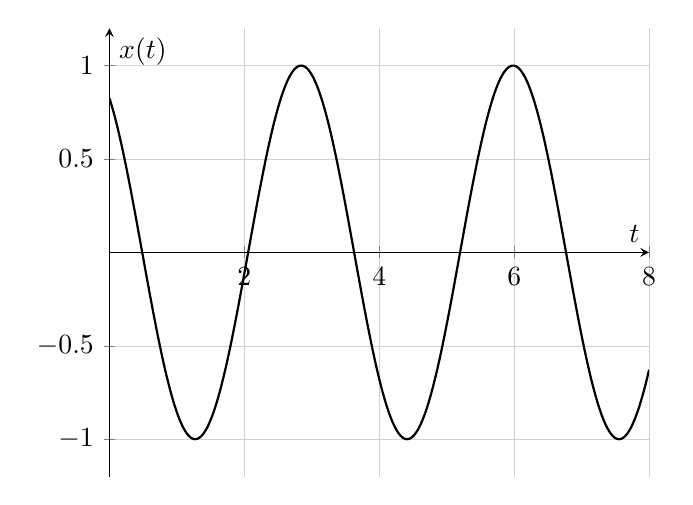
\begin{tikzpicture}
\begin{axis}[
  xlabel={$t$},
  ylabel={$x(t)$},
  axis lines=middle,
  xmin=0, xmax=8,
  ymin=-1.2, ymax=1.2,
  samples=400,
  domain=0:8,
  grid=both,
  grid style={line width=.1pt, draw=gray!25},
  major grid style={line width=.2pt, draw=gray!35},
]
% Esempio: C=1, omega=2, phi=0.6
\addplot[thick] {cos(deg(2*x + 0.6))};
\end{axis}
\end{tikzpicture}
\end{center}


% Richiede: \usepackage{tikz} \usepackage{pgfplots} \pgfplotsset{compat=1.18}


\textbf{Caso (iii): \(\gamma<\omega\) (sottosmorzato)}

Consideriamo
\[
\ddot x(t)+2\gamma\,\dot x(t)+\omega^2 x(t)=0,
\qquad \gamma,\omega>0,
\qquad \gamma<\omega.
\]
Cerchiamo una soluzione del tipo \(x(t)=e^{\lambda t}\). Sostituendo:
\[
\dot x=\lambda e^{\lambda t},\qquad \ddot x=\lambda^2 e^{\lambda t},
\]
si ottiene
\[
\lambda^2 e^{\lambda t}+2\gamma\lambda e^{\lambda t}+\omega^2 e^{\lambda t}=0.
\]
Poiché \(e^{\lambda t}\neq 0\), segue l'equazione caratteristica
\[
\lambda^2+2\gamma\lambda+\omega^2=0.
\]
Le radici sono
\[
\lambda_{\pm}=-\gamma\pm\sqrt{\gamma^2-\omega^2}.
\]
Nel caso \(\gamma<\omega\) vale \(\gamma^2-\omega^2<0\), dunque
\[
\sqrt{\gamma^2-\omega^2}=i\sqrt{\omega^2-\gamma^2}.
\]
Ponendo
\[
\Omega=\sqrt{\omega^2-\gamma^2}>0,
\]
si ottiene
\[
\lambda_{\pm}=-\gamma\pm i\Omega\in\mathbb{C}.
\]

\medskip
\textbf{Soluzione generale (forma complessa).}
Due soluzioni sono \(e^{\lambda_+ t}\) ed \(e^{\lambda_- t}\), quindi
\[
x(t)=A e^{(-\gamma+i\Omega)t}+B e^{(-\gamma-i\Omega)t}.
\]
Raccogliendo \(e^{-\gamma t}\):
\[
x(t)=e^{-\gamma t}\Bigl(A e^{i\Omega t}+B e^{-i\Omega t}\Bigr).
\]

\medskip
\textbf{Passaggio alla forma reale.}
Usiamo le formule di Eulero
\[
e^{i\Omega t}=\cos(\Omega t)+i\sin(\Omega t),\qquad
e^{-i\Omega t}=\cos(\Omega t)-i\sin(\Omega t).
\]
Scegliendo coefficienti tali da ottenere una soluzione reale (equivalentemente, prendendo \(B=\overline{A}\)), l'espressione tra parentesi diventa una combinazione reale di \(\cos(\Omega t)\) e \(\sin(\Omega t)\). Quindi esistono \(C_1,C_2\in\mathbb{R}\) tali che
\[
x(t)=e^{-\gamma t}\Bigl(C_1\cos(\Omega t)+C_2\sin(\Omega t)\Bigr).
\]
Questa forma si riscrive in ampiezza-fase: esistono \(C\ge 0\) e \(\varphi\in\mathbb{R}\) tali che
\[
C_1=C\cos\varphi,\qquad C_2=-C\sin\varphi,
\]
e dunque
\[
x(t)=C e^{-\gamma t}\cos(\Omega t+\varphi).
\]
Questa è un'oscillazione armonica a pulsazione \(\Omega\) con ampiezza modulata dall'inviluppo esponenziale \(e^{-\gamma t}\).

\begin{center}
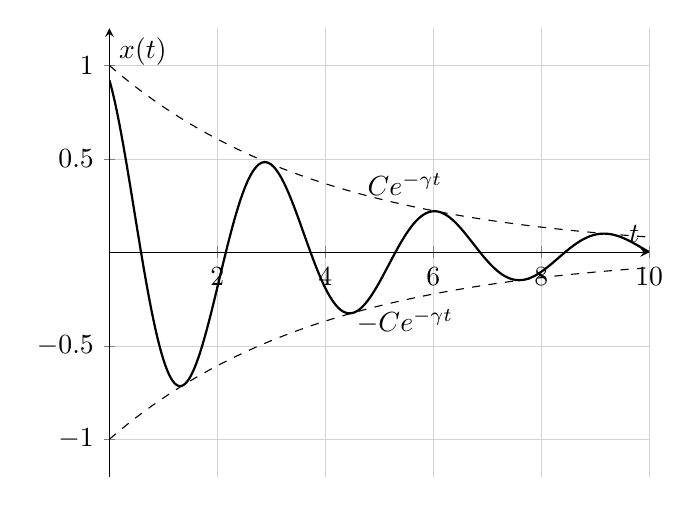
\begin{tikzpicture}
\begin{axis}[
  xlabel={$t$},
  ylabel={$x(t)$},
  axis lines=middle,
  xmin=0, xmax=10,
  ymin=-1.2, ymax=1.2,
  samples=600,
  domain=0:10,
  grid=both,
  grid style={line width=.1pt, draw=gray!25},
  major grid style={line width=.2pt, draw=gray!35},
]
% Esempio numerico: C=1, gamma=0.25, Omega=2, phi=0.4
\addplot[thick] {exp(-0.25*x)*cos(deg(2*x+0.4))};
\addplot[dashed] {exp(-0.25*x)}
  node[pos=0.55, above] {$Ce^{-\gamma t}$};

\addplot[dashed] {-exp(-0.25*x)}
  node[pos=0.55, below] {$-Ce^{-\gamma t}$};
\end{axis}
\end{tikzpicture}
\end{center}
Possiamo riassumere quanto ottenuto finora:
\begin{itemize}
\item \(\gamma=0\) \(\Rightarrow\) nessun attrito: la molla è un oscillatore armonico.

\item \(\gamma>\omega\) \(\Rightarrow\) attrito forte: nessuna oscillazione (oscillatore armonico fortemente smorzato).

\item \(\gamma<\omega\) \(\Rightarrow\) oscillatore che viene smorzato nel tempo dall'attrito \(\bigl(\text{ampiezza}(t)=C e^{-\gamma t}\bigr)\).
\end{itemize}

\begin{oss}{}
Data un'equazione differenziale del \(2^\circ\) ordine possiamo scrivere un sistema di 2 equazioni differenziali del primo ordine ad essa equivalente. Impongo \(x_1=x\), \(x_2=\dot x\).

\[
\ddot x=-2\gamma \dot x-\omega^2 x
\iff
\begin{cases}
\dot x_1=\dot x=x_2,\\
\dot x_2=-2\gamma x_2-\omega^2 x_1.
\end{cases}
\]

\[
\iff\
\frac{d}{dt}
\begin{pmatrix}
x_1\\
x_2
\end{pmatrix}
=
\begin{pmatrix}
0 & 1\\
-\omega^2 & -2\gamma
\end{pmatrix}
\begin{pmatrix}
x_1\\
x_2
\end{pmatrix}.
\]

Notiamo che gli autovalori della matrice
\[
A=
\begin{pmatrix}
0 & 1\\
-\omega^2 & -2\gamma
\end{pmatrix}
\]
sono proprio le radici del polinomio caratteristico di
\[
\ddot x+2\gamma \dot x+\omega^2 x=0,
\qquad\text{ovvero}\qquad
p_A(\lambda)=p(\lambda).
\]
\end{oss}

\textbf{Oscillatore armonico smorzato con forzante periodica}

Consideriamo l’equazione
\[
\ddot{x}+2\gamma \dot{x}+\omega^2 x = F\cos(\Omega t),
\]
dove \(F\) è l’ampiezza della forzante e \(\Omega\) la sua pulsazione.

Poiché l’equazione è lineare, la soluzione generale della non omogenea è somma di una soluzione generale dell’omogenea e di una particolare:
\[
x(t)=x_0(t)+x_p(t),
\]
con
\[
\ddot{x}_0+2\gamma \dot{x}_0+\omega^2 x_0=0,
\qquad
\ddot{x}_p+2\gamma \dot{x}_p+\omega^2 x_p=F\cos(\Omega t).
\]

\medskip
\textbf{Caso \(\gamma=0\).}
L’equazione diventa
\[
\ddot{x}+\omega^2 x = F\cos(\Omega t).
\]
Cerchiamo una particolare del tipo \(x_p(t)=D\cos(\Omega t)\). Allora
\[
\ddot{x}_p(t)=-D\Omega^2\cos(\Omega t),
\]
e sostituendo:
\[
-D\Omega^2\cos(\Omega t)+\omega^2 D\cos(\Omega t)=F\cos(\Omega t)
\quad\Rightarrow\quad
D(\omega^2-\Omega^2)=F.
\]
Quindi, se \(\Omega\neq\omega\),
\[
D=\frac{F}{\omega^2-\Omega^2},
\qquad
x_p(t)=\frac{F}{\omega^2-\Omega^2}\cos(\Omega t).
\]
La soluzione generale è allora
\[
x(t)=C\cos(\omega t+\varphi)+\frac{F}{\omega^2-\Omega^2}\cos(\Omega t),
\]
dove \(C\) e \(\varphi\) si determinano dalle condizioni iniziali. In particolare, imponendo
\(x(0)=x_0\) e \(\dot{x}(0)=v_0\),
\[
x_0=C\cos\varphi+\frac{F}{\omega^2-\Omega^2}\cos(0),
\]
\[
v_0=-\omega C\sin\varphi-\frac{F}{\omega^2-\Omega^2}\,\Omega\sin(0).
\]

\medskip
\textbf{Caso \(\gamma\neq 0\).}
Proviamo una particolare del tipo
\[
x_p(t)=D\cos(\Omega t+\beta).
\]
Allora
\[
\dot{x}_p(t)=-D\Omega\sin(\Omega t+\beta),
\qquad
\ddot{x}_p(t)=-D\Omega^2\cos(\Omega t+\beta).
\]
Sostituendo nell’equazione:
\[
(\omega^2-\Omega^2)D\cos(\Omega t+\beta)-2\gamma\Omega D\sin(\Omega t+\beta)=F\cos(\Omega t).
\]
Usando
\[
\cos(\Omega t+\beta)=\cos(\Omega t)\cos\beta-\sin(\Omega t)\sin\beta,
\]
\[
\sin(\Omega t+\beta)=\sin(\Omega t)\cos\beta+\cos(\Omega t)\sin\beta,
\]
si ottiene
\[
\cos(\Omega t)\,D\bigl[(\omega^2-\Omega^2)\cos\beta-2\gamma\Omega\sin\beta\bigr]
+\sin(\Omega t)\,D\bigl[-(\omega^2-\Omega^2)\sin\beta-2\gamma\Omega\cos\beta\bigr] =
\]
\[
=F\cos(\Omega t)+0\cdot\sin(\Omega t).
\]
Eguagliando i coefficienti di \(\cos(\Omega t)\) e \(\sin(\Omega t)\) si ottiene il sistema
\[
\begin{cases}
D\bigl[(\omega^2-\Omega^2)\cos\beta-2\gamma\Omega\sin\beta\bigr]=F,\\[4pt]
D\bigl[(\omega^2-\Omega^2)\sin\beta+2\gamma\Omega\cos\beta\bigr]=0.
\end{cases}
\]
Dalla seconda equazione:
\[
(\omega^2-\Omega^2)\sin\beta+2\gamma\Omega\cos\beta=0
\quad\Rightarrow\quad
\tan\beta=-\dfrac{2\gamma\Omega}{\omega^2-\Omega^2}
=\dfrac{2\gamma\Omega}{\Omega^2-\omega^2}.
\]
Inoltre, elevando al quadrato e sommando le due equazioni del sistema si ricava
\[
D^2\bigl[(\omega^2-\Omega^2)^2+(2\gamma\Omega)^2\bigr]=F^2
\quad\Rightarrow\quad
D=\frac{F}{\sqrt{(\omega^2-\Omega^2)^2+(2\gamma\Omega)^2}}.
\]

\medskip
\textbf{Soluzione generale (caso \(\gamma<\omega\)).}
Se \(\gamma<\omega\), la soluzione dell’omogenea è
\[
x_0(t)=C\,e^{-\gamma t}\cos\!\bigl(\sqrt{\omega^2-\gamma^2}\,t+\varphi\bigr),
\]
e quindi la soluzione generale della forzata è
\[
x(t)=C\,e^{-\gamma t}\cos\!\bigl(\sqrt{\omega^2-\gamma^2}\,t+\varphi\bigr)
+ D\cos(\Omega t+\beta),
\]
con
\[
D=\frac{F}{\sqrt{(\omega^2-\Omega^2)^2+(2\gamma\Omega)^2}},
\qquad
\tan\beta=\frac{2\gamma\Omega}{\Omega^2-\omega^2}.
\]

\begin{oss}{}
Nel caso \(\gamma>0\) il termine transiente \(x_0(t)\) decade esponenzialmente, quindi
\[
\lim_{t\to+\infty} x(t) = \text{(componente forzata)} \quad\Rightarrow\quad
x(t)\sim D\cos(\Omega t+\beta)\ \ \text{per } t\to+\infty.
\]
In altre parole, il sistema “dimentica” le condizioni iniziali: a regime resta solo l’oscillazione alla frequenza della forzante.
\end{oss}
